\subsection{Operazioni Preliminari}
Per prima cosa si procede al montaggio dell'apparato sperimentale, formato da un bilanciere collegato ad un supporto con molla, come in figura (x). Successivamente, si procede a ruotare il bilanciere di 180\(^\circ\) rispetto alla posizione di equilibrio. Disponendo un dinamometro ortogonalmente al bilanciere e parallelamente al suolo, è stato possibile misurare la forza di richiamo della molla in corrispondenza di diversi valori della distanza $r$ del punto di applicazione del dinamometro dal centro del bilanciere. La disposizione del dinamometro ci consente di calcolare il modulo del momento della forza di richiamo semplicemente come 
\begin{equation}
    M = F \cdot r
\end{equation}
I dati relativi alle distanze e alle forze di richiamo misurate sono contenuti nelle seguenti tabelle:

\begin{table}[H]
	\centering
	\begin{tabular}{|c|c|}
		\hline
		& \textbf{r $[cm]$ } \\
		\hline
		  $r_1$ & $30.00\pm 0.05$ \\
		$r_2$ & $25.00\pm 0.05$ \\
		$r_3$ & $20.00\pm 0.05$ \\
		$r_4$ & $15.00\pm 0.05$ \\
		$r_5$ & $10.00\pm 0.05$ \\
            $r_6$ & $5.00 \pm 0.05$ \\
		\hline
	\end{tabular}
	\caption{Distanze $r$ del punto di applicazione del dinamometro dal centro del bilanciere.}
	\label{tab:}
\end{table}

\begin{table}[H]
	\centering
	\begin{tabular}{|c|}
		\hline
		\textbf{F $[N]$} \\
		\hline
		$0.175\pm 0.025$ \\
		$0.225\pm 0.025$ \\
		$0.275\pm 0.025$ \\
		$0.375\pm 0.025$ \\
		$0.550\pm 0.025$ \\
            $1.10 \pm 0.03$ \\
		\hline
	\end{tabular}
	\caption{Forze di richiamo $F$ al variare della distanza $r$.}
	\label{tab:}
\end{table}

In corrispondenza dei valori di $r$ ed $F$ misurati, si ottengono i valori del momento $M$:

\begin{table}[H]
	\centering
	\begin{tabular}{|c|}
		\hline
		\textbf{M $[N*m]$} \\
		\hline
		$(5.25\pm 0.04)10^{-2}$ \\
		$(5.63\pm 0.04)10^{-2}$ \\
		$(5.50\pm 0.03)10^{-2}$ \\
		$(5.63\pm 0.03)10^{-2}$ \\
		$(5.50\pm 0.03)10^{-2}$ \\
            $(5.50 \pm 0.01)10^{-2}$ \\
		\hline
	\end{tabular}
	\caption{Momento $M$ della forza di richiamo al variare della distanza $r$.}
	\label{tab:}
\end{table}

I valori di $M$ sono stati calcolati utilizzando la formula (24), arrotondandoli al numero minimo di cifre significative tra quelle dei fattori $r$ ed $F$, pari a tre. Le incertezze su $M$ sono state ottenute al seguente modo:
\begin{itemize}
    \item Dalla legge di propagazione dell'errore (17) si ottiene, nel nostro caso: 
    \begin{equation}
        \frac{\delta M}{|M|} = \frac{\delta F}{|F|} + \frac{\delta r}{|r|}
    \end{equation}
    \item Si calcola l'incertezza assoluta:
    \begin{equation}
        \delta M = \frac{\delta M}{|M|} \cdot |M|
    \end{equation}
\end{itemize}

Possiamo infine calcolare la migliore stima di $M$ come media dei valori riportati in tabella (4) e l'incertezza associata come deviazione standard della media:

\begin{itemize}
    \item Stima migliore per $M$:
    \begin{equation}
        M_{best} = \frac{1}{N}\sum_{i=1}^{N} x_i
    \end{equation}
    dove $N$ è il numero di misurazioni disponibili, $x_i$ i rispettivi valori. Nel nostro caso,
    \begin{equation}
        M_{best} = 0.055 \ Nm
    \end{equation}
    \item Deviazione standard della media:
    \begin{equation}
        \sigma_{\bar{x}} = \sigma_x/\sqrt{N}
    \end{equation}
    ove $\bar{x} = M_{best}$ e $\sigma_x$ indica la deviazione standard dei valori di $M$. Nel nostro caso:
    \begin{equation}
        \sigma_{\bar{x}} = 0.001 \ Nm
    \end{equation}
\end{itemize}
A questo punto, è possibile sfruttare l'equazione (6) per stimare il modulo di $K$:
\begin{equation}
    K = \frac{M}{\pi} 
\end{equation}
otteniamo così la seguente conclusione: 
\begin{itemize}
    \item $K = 0.018 \ Nm$. 
    \item $\delta K = \frac{1}{\pi}\cdot \delta M = 0.001 \  Nm$
\end{itemize}

\subsection{Parte I: Misura del momento d'inerzia di un corpo rigido}
Scopo della presente sezione è la misurazione del momento d'inerzia di una coppia di masse approssimativamente uguali, disposte simmetricamente rispetto all'asse perpendicolare al bilanciere e passante per il suo centro. Dopo aver posizionato le masse sul bilanciere in posizione simmetrica, si procede a determinare e registrare la posizione di equilibrio del sistema. Ruotando il bilanciere di un angolo pari a $\frac{\pi}{2}$ rispetto alla posizione di equilibrio, il sistema viene lasciato in oscillazione libera. Si procede così alla misurazione del tempo corrispondente a 5 oscillazioni a partire dal primo passaggio dalla posizione di equilibrio. La misura è stata ripetuta 4 volte alternando le rotazioni in senso orario e antiorario, in maniera tale da poter ricavare una stima accettabile del periodo di oscillazione. La procedura è stata ripetuta 6 volte, riducendo ad ogni passaggio la distanza delle due masse dal centro secondo quanto riportato in tabella (2).

\begin{table}[H]
	\centering
	\begin{tabular}{|c|c|c|c|c|c|}
		\hline
            Distanze & $T_1$ [s] & $T_2$ [s]& $T_3$ [s]& $T_4$ [s] & $\delta T$ [s]\\
            \hline
            $r_1$ & 47.92 & 47.75 & 47.72 & 47.72 & 0.01\\
            \hline
            $r_2$ & 40.40 & 40.44 & 40.50 & 40.44 & 0.01\\
            \hline
            $r_3$ & 33.77 & 33.65 & 33.58 & 33.60 & 0.01\\
            \hline
            $r_4$ & 26.87 & 26.87 & 26.77 & 26.70 & 0.01\\
            \hline
            $r_5$ & 20.73 & 20.77 & 20.77 & 20.75 & 0.01\\
            \hline
            $r_6$ & 16.00 & 16.14 & 16.16 & 16.05 & 0.01\\
            \hline
        \end{tabular}
	\caption{Tabella dei periodi in funzione delle distanze dal centro del bilanciere.}
	\label{tab:}
\end{table}

Poichè per ogni distanza abbiamo a disposizione solo poche misure del periodo $T$ che si ripetono, possiamo stimare questo valore al seguente modo:
\begin{itemize}
    \item Stima del periodo:
    \begin{equation}
        T_{best} = \frac{T_{max} + T_{min}}{2}
    \end{equation}
    dove $T_{max}$ è il periodo più alto e $T_{min}$ quello più basso rispetto ad una distanza fissata.
    \item Stima dell'incertezza con il metodo della semidispersione: 
    \begin{equation}
        \delta T = \frac{T_{max} - T_{min}}{2}
    \end{equation}
\end{itemize}

La tabella che segue riporta i valori numerici delle stime ottenute tenendo conto delle (32) e (33):

\begin{table}[H]
	\centering
	\begin{tabular}{|c|}
		\hline
		\textbf{I $[kg \cdot m^2]$} \\
		\hline
		$47.82\pm 0.10$ \\
		$40.45\pm 0.05$ \\
		$33.68\pm 0.10$ \\
		$26.79\pm 0.09$ \\
		$20.75\pm 0.02$ \\
            $16.08 \pm 0.08$ \\
		\hline
	\end{tabular}
	\caption{Periodi di oscillazione.}
	\label{tab:}
\end{table}


A questo punto, mediante semplici calcoli, è possibile ricavare una stima del momento d'inerzia dalla formula (3):
\begin{equation}
    I = \frac{K \cdot T^2}{4\pi^2}
\end{equation} 
Osserviamo che i valori ricavati per $I$ misurano il momento d'inerzia del sistema bilanciere-masse e pertanto contengono un termine addizionale rappresentato dal momento d'inerzia del bilanciere vuoto $I_a = 0.01 \pm 0.01 \ kg \cdot m^2$, che va sottratto dai valori ottenuti dalla (34), per ottenere il momento d'inerzia delle sole masse. La propagazione dell'incertezza su $I$ è stata valutata con il metodo dei differenziali (Legge (17)):

\begin{equation}
    \delta I = \frac{T^2 \delta K + 2 KT \delta T}{4\pi^2} + \delta I_a
\end{equation}

La tabella che segue riporta i valori numerici delle stime ottenute tenendo conto delle (34) e (35):

\begin{table}[H]
	\centering
	\begin{tabular}{|c|}
		\hline
		\textbf{I $[kg \cdot m^2]$} \\
		\hline
		$1.0\pm 0.2$ \\
		$0.72\pm 0.01$ \\
		$0.50\pm 0.01$ \\
		$0.31\pm 0.01$ \\
		$0.19\pm 0.01$ \\
            $0.11 \pm 0.01$ \\
		\hline
	\end{tabular}
	\caption{Momento d'inerzia al variare della distanza dal centro del bilanciere.}
	\label{tab:}
\end{table}

Poichè $K$ e $T$ sono riportati rispettivamente con 2 e 4 cifre significative, il momento di inerzia $I$ è stato riportato con 2 cifre significative.

Di seguito viene riportato il grafico di $I$ in funzione di $d^2$.

\begin{figure}[h]
    \centering
    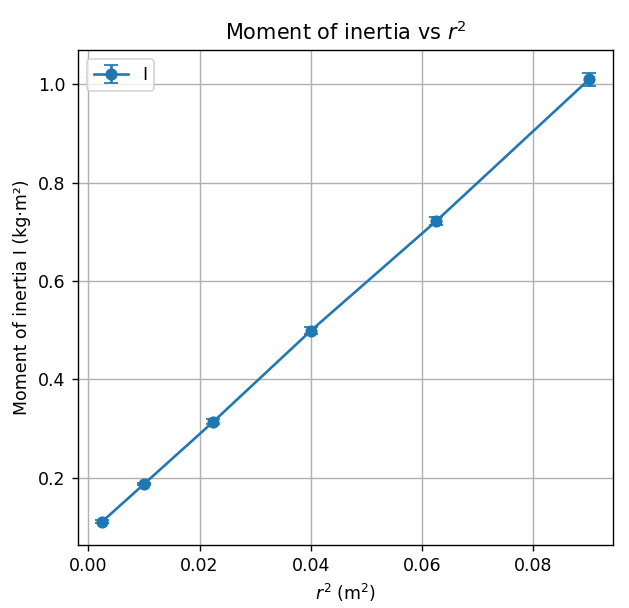
\includegraphics[width=0.6\textwidth]{Latex/graph_1.png}
    \caption{Grafico del momento d'inerzia in funzione del quadrato della distanza}
    \label{fig:etichetta}
\end{figure}

\subsection{Parte II: Verifica Del Teorema di Huygens-Steiner}
Scopo della presente sezione è verificare che il momento d'inerzia di un disco rispetto ad un asse parallelo ad un asse baricentrico e a distanza $d$ da quest'ultimo dipende linearmente da $d^2$, coerentemente con il teorema di Huygens-Steiner. Un disco forato è stato montato al supporto con molla, utilizzando preliminarmente il foro centrale. Ruotando il disco di un angolo $\frac{\pi}{2}$ rispetto alla posizione di equilibrio, si procede con la misurazione del periodo corrispondente a 5 oscillazioni, contate azionando il cronometro in corrispondenza del primo passaggio dalla posizione di equilibrio fissata precedentemente. La misura è stata ripetuta per 4 volte, ruotando alternativamente il disco in senso orario e antiorario. La procedura appena descritta è stata ripetuta variando la posizione del disco utilizzando i fori praticati sulla sua superficie. Le distanze utilizzate sono riportate nella seguente tabella:

\begin{table}[H]
	\centering
	\begin{tabular}{|c|}
		\hline
		\textbf{d $[cm]$} \\
		\hline
		$2.05\pm 0.05$ \\
		$4.05\pm 0.05$ \\
		$6.05\pm 0.05$ \\
		$8.05\pm 0.05$ \\
            $10.05 \pm 0.05$ \\
		\hline
	\end{tabular}
	\caption{Distanze dell'asse rispetto all'asse baricentrico ortogonale al disco.}
	\label{tab:}
\end{table}

Il momento d'inerzia del disco rispetto agli assi corrispondenti alle distanze riportate in tabella è stato calcolando seguendo la stessa procedura della prima parte, ottenendo i seguenti risultati:

\begin{table}[H]
	\centering
	\begin{tabular}{|c|}
		\hline
		\textbf{I $[kg \cdot m^2]$} \\
		\hline
		$0.316\pm 0.005$ \\
		$0.319\pm 0.004$ \\
		$0.352\pm 0.005$ \\
		$0.472\pm 0.017$ \\
            $0.535 \pm 0.009$ \\
		\hline
	\end{tabular}
	\caption{Momenti d'inerzia. Il momento d'inerzia rispetto al baricentro è $I_0 = 0.291\pm 0.006 (kg \cdot m^2)$}
	\label{tab:}
\end{table}

Di seguito, riportiamo i valori del momento d'inerzia $I$ in funzione del quadrato della distanza $d^2$ fra il foro centrale e quello utilizzato per il fissaggio del disco. 

\begin{figure}[H]
    \centering
    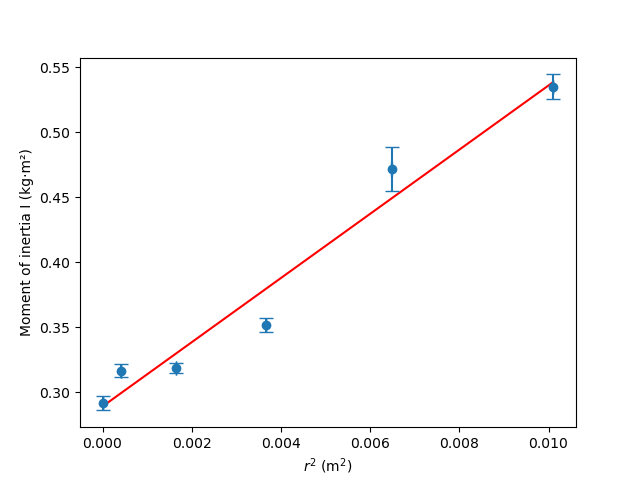
\includegraphics[width=0.6\textwidth]{Latex/graph_2.png}
    \caption{Grafico del momento d'inerzia in funzione del quadrato della distanza}
    \label{fig:etichetta}
\end{figure}